\documentclass[twoside]{book}

% Packages required by doxygen
\usepackage{fixltx2e}
\usepackage{calc}
\usepackage{doxygen}
\usepackage{graphicx}
\usepackage[utf8]{inputenc}
\usepackage{makeidx}
\usepackage{multicol}
\usepackage{multirow}
\PassOptionsToPackage{warn}{textcomp}
\usepackage{textcomp}
\usepackage[nointegrals]{wasysym}
\usepackage[table]{xcolor}

% NLS support packages
Portuguese
% Font selection
\usepackage[T1]{fontenc}
\usepackage{mathptmx}
\usepackage[scaled=.90]{helvet}
\usepackage{courier}
\usepackage{amssymb}
\usepackage{sectsty}
\renewcommand{\familydefault}{\sfdefault}
\allsectionsfont{%
  \fontseries{bc}\selectfont%
  \color{darkgray}%
}
\renewcommand{\DoxyLabelFont}{%
  \fontseries{bc}\selectfont%
  \color{darkgray}%
}
\newcommand{\+}{\discretionary{\mbox{\scriptsize$\hookleftarrow$}}{}{}}

% Page & text layout
\usepackage{geometry}
\geometry{%
  a4paper,%
  top=2.5cm,%
  bottom=2.5cm,%
  left=2.5cm,%
  right=2.5cm%
}
\tolerance=750
\hfuzz=15pt
\hbadness=750
\setlength{\emergencystretch}{15pt}
\setlength{\parindent}{0cm}
\setlength{\parskip}{0.2cm}
\makeatletter
\renewcommand{\paragraph}{%
  \@startsection{paragraph}{4}{0ex}{-1.0ex}{1.0ex}{%
    \normalfont\normalsize\bfseries\SS@parafont%
  }%
}
\renewcommand{\subparagraph}{%
  \@startsection{subparagraph}{5}{0ex}{-1.0ex}{1.0ex}{%
    \normalfont\normalsize\bfseries\SS@subparafont%
  }%
}
\makeatother

% Headers & footers
\usepackage{fancyhdr}
\pagestyle{fancyplain}
\fancyhead[LE]{\fancyplain{}{\bfseries\thepage}}
\fancyhead[CE]{\fancyplain{}{}}
\fancyhead[RE]{\fancyplain{}{\bfseries\leftmark}}
\fancyhead[LO]{\fancyplain{}{\bfseries\rightmark}}
\fancyhead[CO]{\fancyplain{}{}}
\fancyhead[RO]{\fancyplain{}{\bfseries\thepage}}
\fancyfoot[LE]{\fancyplain{}{}}
\fancyfoot[CE]{\fancyplain{}{}}
\fancyfoot[RE]{\fancyplain{}{\bfseries\scriptsize Gerado em Sexta, 19 de Agosto de 2016 23\+:33\+:30 para Home\+Stark por Doxygen }}
\fancyfoot[LO]{\fancyplain{}{\bfseries\scriptsize Gerado em Sexta, 19 de Agosto de 2016 23\+:33\+:30 para Home\+Stark por Doxygen }}
\fancyfoot[CO]{\fancyplain{}{}}
\fancyfoot[RO]{\fancyplain{}{}}
\renewcommand{\footrulewidth}{0.4pt}
\renewcommand{\chaptermark}[1]{%
  \markboth{#1}{}%
}
\renewcommand{\sectionmark}[1]{%
  \markright{\thesection\ #1}%
}

% Indices & bibliography
\usepackage{natbib}
\usepackage[titles]{tocloft}
\setcounter{tocdepth}{3}
\setcounter{secnumdepth}{5}
\makeindex

% Hyperlinks (required, but should be loaded last)
\usepackage{ifpdf}
\ifpdf
  \usepackage[pdftex,pagebackref=true]{hyperref}
\else
  \usepackage[ps2pdf,pagebackref=true]{hyperref}
\fi
\hypersetup{%
  colorlinks=true,%
  linkcolor=blue,%
  citecolor=blue,%
  unicode%
}

% Custom commands
\newcommand{\clearemptydoublepage}{%
  \newpage{\pagestyle{empty}\cleardoublepage}%
}


%===== C O N T E N T S =====

\begin{document}

% Titlepage & ToC
\hypersetup{pageanchor=false,
             bookmarks=true,
             bookmarksnumbered=true,
             pdfencoding=unicode
            }
\pagenumbering{roman}
\begin{titlepage}
\vspace*{7cm}
\begin{center}%
{\Large Home\+Stark \\[1ex]\large 1.\+0 }\\
\vspace*{1cm}
{\large Gerado por Doxygen 1.8.8}\\
\vspace*{0.5cm}
{\small Sexta, 19 de Agosto de 2016 23:33:30}\\
\end{center}
\end{titlepage}
\clearemptydoublepage
\tableofcontents
\clearemptydoublepage
\pagenumbering{arabic}
\hypersetup{pageanchor=true}

%--- Begin generated contents ---
\chapter{R\+E\+A\+D\+M\+E}
\label{md_README}
\hypertarget{md_README}{}
\#\+Projeto Home\+Stark \+:coffee\+: 

 $\vert$ $\vert$ $\vert$ $\vert$ \+\_\+\+\_\+\+\_\+ \+\_\+ \+\_\+\+\_\+ \+\_\+\+\_\+\+\_\+ \+\_\+\+\_\+\+\_\+/ \+\_\+\+\_\+\+\_\+$\vert$$\vert$ $\vert$\+\_\+ \+\_\+\+\_\+ \+\_\+ \+\_\+ \+\_\+\+\_\+$\vert$ $\vert$ \+\_\+\+\_\+ $\vert$ $\vert$\+\_\+$\vert$ $\vert$/ \+\_\+ $|$ '\+\_\+ {\ttfamily \+\_\+ \textbackslash{} / \+\_\+ \textbackslash{}\+\_\+\+\_\+\+\_\+ \textbackslash{}$\vert$ \+\_\+\+\_\+/ \+\_\+} $\vert$ '\+\_\+\+\_\+$\vert$ $\vert$/ / $\vert$ \+\_\+ $\vert$ (\+\_\+) $\vert$ $\vert$ $\vert$ $\vert$ $\vert$ $\vert$ \+\_\+\+\_\+/\+\_\+\+\_\+\+\_\+) $\vert$ $\vert$$\vert$ (\+\_\+$\vert$ $\vert$ $\vert$ $\vert$ $<$ $\vert$\+\_\+$\vert$ $\vert$\+\_\+$\vert$\+\_\+\+\_\+\+\_\+/$\vert$\+\_\+$\vert$ $\vert$\+\_\+$\vert$ $\vert$\+\_\+$\vert$\+\_\+\+\_\+\+\_\+$\vert$\+\_\+\+\_\+\+\_\+\+\_\+/ \+\_\+\+\_\+\+\_\+\+\_\+,\+\_\+$\vert$\+\_\+$\vert$ $\vert$\+\_\+$\vert$\+\_\+\textbackslash{}

$>$make T\+A\+R\+G\+E\+T=srf06-\/cc26xx

Desenvolvedor\+: Ânderson Ignácio da Silva

Projeto de T\+C\+C para criação de uma rede mesh 6\+Lo\+W\+P\+A\+N utilizando o target cc2650 da Texas Instruments. O dispositivo será capaz de se conectar a uma rede mesh 6\+Lo\+W\+P\+A\+N, comunicando via M\+Q\+T\+T-\/\+S\+N com broker remoto e local através de um interface de gestão/configuração.

Características\+:
\begin{DoxyItemize}
\item \mbox{[} \mbox{]} Suporte completo a M\+Q\+T\+T-\/\+S\+N
\item \mbox{[} \mbox{]} D\+T\+L\+S sobre U\+D\+P
\item \mbox{[} \mbox{]} Informação ao border router sobre o nó
\item \mbox{[} \mbox{]} Comunicação com periféricos e afins
\item \mbox{[} \mbox{]} Documentação em Doxygen
\end{DoxyItemize}

Nomenclaturas\+:

E\+T\+X (expected transmission count) = Medidor de qualidade de caminho entre dois nós em um pacote wireless de rede. Basicamente esse núme ro indica o número esperado de transmissões de um pacote necessária s para que não haja erro na recepção no destino. 
\chapter{Índice dos componentes}
\section{Estruturas de dados}
Lista das estruturas de dados com uma breve descrição\+:\begin{DoxyCompactList}
\item\contentsline{section}{\hyperlink{structconnect__packet__t}{connect\+\_\+packet\+\_\+t} \\*Estrutura de pacotes M\+Q\+T\+T-\/\+S\+N do tipo C\+O\+N\+N\+E\+C\+T }{\pageref{structconnect__packet__t}}{}
\item\contentsline{section}{\hyperlink{structmqtt__sn__t}{mqtt\+\_\+sn\+\_\+t} \\*Estrutura de conexão ao broker M\+Q\+T\+T-\/\+S\+N }{\pageref{structmqtt__sn__t}}{}
\item\contentsline{section}{\hyperlink{structmqtt__sn__task__t}{mqtt\+\_\+sn\+\_\+task\+\_\+t} \\*Estrutura de tarefa de fila M\+Q\+T\+T-\/\+S\+N }{\pageref{structmqtt__sn__task__t}}{}
\item\contentsline{section}{\hyperlink{structnode}{node} \\*Estrutura de fila M\+Q\+T\+T-\/\+S\+N }{\pageref{structnode}}{}
\item\contentsline{section}{\hyperlink{structpublish__packet__t}{publish\+\_\+packet\+\_\+t} \\*Estruturas para o bind de topic e short topic id }{\pageref{structpublish__packet__t}}{}
\item\contentsline{section}{\hyperlink{structregister__packet__t}{register\+\_\+packet\+\_\+t} \\*Estrutura de pacotes M\+Q\+T\+T-\/\+S\+N do tipo R\+E\+G\+I\+S\+T\+E\+R }{\pageref{structregister__packet__t}}{}
\end{DoxyCompactList}

\chapter{Índice dos ficheiros}
\section{Lista de ficheiros}
Lista de todos os ficheiros documentados com uma breve descrição\+:\begin{DoxyCompactList}
\item\contentsline{section}{\hyperlink{main__core_8c}{main\+\_\+core.\+c} \\*Arquivo principal do código fonte da rede mesh 6\+Lo\+W\+P\+A\+N ~\newline
 Para compilar este código, execute o makefile com o target desejado, por exemplo\+: ~\newline
 {\bfseries \char`\"{}make T\+A\+R\+G\+E\+T=srf06-\/cc26xx\char`\"{}} ~\newline
 Caso não reconheça qual o T\+A\+R\+G\+E\+T correto, utiliza o comando ~\newline
 {\bfseries \char`\"{}make targets\char`\"{}} ~\newline
 para listar os tags disponíveis }{\pageref{main__core_8c}}{}
\item\contentsline{section}{\hyperlink{mqtt__sn_8h}{mqtt\+\_\+sn.\+h} \\*\begin{DoxyVerb}    Conjunto de protótipos e definiçoes do protocolo MQTT-SN
\end{DoxyVerb}
 }{\pageref{mqtt__sn_8h}}{}
\item\contentsline{section}{{\bfseries project-\/conf.\+h} }{\pageref{project-conf_8h}}{}
\item\contentsline{section}{{\bfseries symbols.\+h} }{\pageref{symbols_8h}}{}
\item\contentsline{section}{\hyperlink{syscalls_8c}{syscalls.\+c} \\*System calls }{\pageref{syscalls_8c}}{}
\item\contentsline{section}{aux\+\_\+tools/\hyperlink{sabado__list__old_8h}{sabado\+\_\+list\+\_\+old.\+h} \\*\begin{DoxyVerb}    Conjunto de protótipos e definiçoes do protocolo MQTT-SN
\end{DoxyVerb}
 }{\pageref{sabado__list__old_8h}}{}
\end{DoxyCompactList}

\chapter{Documentação da classe}
\hypertarget{structconnack__packet__t}{\section{Referência à estrutura connack\+\_\+packet\+\_\+t}
\label{structconnack__packet__t}\index{connack\+\_\+packet\+\_\+t@{connack\+\_\+packet\+\_\+t}}
}
\subsection*{Atributos Públicos}
\begin{DoxyCompactItemize}
\item 
\hypertarget{structconnack__packet__t_a392983470536680eeb87165f76ab7296}{uint8\+\_\+t {\bfseries length}}\label{structconnack__packet__t_a392983470536680eeb87165f76ab7296}

\item 
\hypertarget{structconnack__packet__t_a63a96761c52d9ea54c54bef14e35562f}{uint8\+\_\+t {\bfseries type}}\label{structconnack__packet__t_a63a96761c52d9ea54c54bef14e35562f}

\item 
\hypertarget{structconnack__packet__t_ae3c0f8da28cb920a1e382b1192305f15}{uint8\+\_\+t {\bfseries return\+\_\+code}}\label{structconnack__packet__t_ae3c0f8da28cb920a1e382b1192305f15}

\end{DoxyCompactItemize}


A documentação para esta estrutura foi gerada a partir do seguinte ficheiro\+:\begin{DoxyCompactItemize}
\item 
mqtt-\/sn.\+h\end{DoxyCompactItemize}

\hypertarget{structconnect__packet__t}{\section{Referência à estrutura connect\+\_\+packet\+\_\+t}
\label{structconnect__packet__t}\index{connect\+\_\+packet\+\_\+t@{connect\+\_\+packet\+\_\+t}}
}
\subsection*{Atributos Públicos}
\begin{DoxyCompactItemize}
\item 
\hypertarget{structconnect__packet__t_a51228edf71d2c3b0b8d049beea278ad7}{uint8\+\_\+t {\bfseries length}}\label{structconnect__packet__t_a51228edf71d2c3b0b8d049beea278ad7}

\item 
\hypertarget{structconnect__packet__t_a082de55b8377052e1957ff8bad186037}{uint8\+\_\+t {\bfseries type}}\label{structconnect__packet__t_a082de55b8377052e1957ff8bad186037}

\item 
\hypertarget{structconnect__packet__t_a91eb3d6559284c3385ebec9bfeca0ec6}{uint8\+\_\+t {\bfseries flags}}\label{structconnect__packet__t_a91eb3d6559284c3385ebec9bfeca0ec6}

\item 
\hypertarget{structconnect__packet__t_aea7d723928bde83abf3274c4658f6a16}{uint8\+\_\+t {\bfseries protocol\+\_\+id}}\label{structconnect__packet__t_aea7d723928bde83abf3274c4658f6a16}

\item 
\hypertarget{structconnect__packet__t_a274e305934afe0330abdc28131697003}{uint16\+\_\+t {\bfseries duration}}\label{structconnect__packet__t_a274e305934afe0330abdc28131697003}

\item 
\hypertarget{structconnect__packet__t_a141fbc06968f67ba017ce7672a93d893}{char {\bfseries client\+\_\+id} \mbox{[}23\mbox{]}}\label{structconnect__packet__t_a141fbc06968f67ba017ce7672a93d893}

\end{DoxyCompactItemize}


A documentação para esta estrutura foi gerada a partir do seguinte ficheiro\+:\begin{DoxyCompactItemize}
\item 
mqtt-\/sn.\+h\end{DoxyCompactItemize}

\hypertarget{structdisconnect__packet__t}{\section{Referência à estrutura disconnect\+\_\+packet\+\_\+t}
\label{structdisconnect__packet__t}\index{disconnect\+\_\+packet\+\_\+t@{disconnect\+\_\+packet\+\_\+t}}
}
\subsection*{Atributos Públicos}
\begin{DoxyCompactItemize}
\item 
\hypertarget{structdisconnect__packet__t_ae040bbd3cf30dc507447d3c3f03fdd2a}{uint8\+\_\+t {\bfseries length}}\label{structdisconnect__packet__t_ae040bbd3cf30dc507447d3c3f03fdd2a}

\item 
\hypertarget{structdisconnect__packet__t_a666b42d5da2d9c45a37515217f470932}{uint8\+\_\+t {\bfseries type}}\label{structdisconnect__packet__t_a666b42d5da2d9c45a37515217f470932}

\item 
\hypertarget{structdisconnect__packet__t_a4d0f4307f03380c20cfbed4b4a52737a}{uint16\+\_\+t {\bfseries duration}}\label{structdisconnect__packet__t_a4d0f4307f03380c20cfbed4b4a52737a}

\end{DoxyCompactItemize}


A documentação para esta estrutura foi gerada a partir do seguinte ficheiro\+:\begin{DoxyCompactItemize}
\item 
mqtt-\/sn.\+h\end{DoxyCompactItemize}

\hypertarget{structmqtt__sn__callbacks}{\section{Referência à estrutura mqtt\+\_\+sn\+\_\+callbacks}
\label{structmqtt__sn__callbacks}\index{mqtt\+\_\+sn\+\_\+callbacks@{mqtt\+\_\+sn\+\_\+callbacks}}
}
\subsection*{Campos de Dados}
\begin{DoxyCompactItemize}
\item 
\hypertarget{structmqtt__sn__callbacks_a52516850dd00bb113cbface2a0b2a9d8}{void($\ast$ \hyperlink{structmqtt__sn__callbacks_a52516850dd00bb113cbface2a0b2a9d8}{pub\+\_\+recv} )(struct \hyperlink{structmqtt__sn__connection}{mqtt\+\_\+sn\+\_\+connection} $\ast$mqc, const uip\+\_\+ipaddr\+\_\+t $\ast$source\+\_\+addr, const uint8\+\_\+t $\ast$data, uint16\+\_\+t datalen)}\label{structmqtt__sn__callbacks_a52516850dd00bb113cbface2a0b2a9d8}

\begin{DoxyCompactList}\small\item\em Called when a packet has been received by the mqtt\+\_\+sn module or other event needs handled. \end{DoxyCompactList}\item 
\hypertarget{structmqtt__sn__callbacks_af8239d3686b4a4d0e2a6c1d4196dc16a}{void($\ast$ {\bfseries pingreq\+\_\+recv} )(struct \hyperlink{structmqtt__sn__connection}{mqtt\+\_\+sn\+\_\+connection} $\ast$mqc, const uip\+\_\+ipaddr\+\_\+t $\ast$source\+\_\+addr, const uint8\+\_\+t $\ast$data, uint16\+\_\+t datalen)}\label{structmqtt__sn__callbacks_af8239d3686b4a4d0e2a6c1d4196dc16a}

\item 
\hypertarget{structmqtt__sn__callbacks_ae0badde8eb4b728bf6eac9e562103a86}{void($\ast$ {\bfseries pingresp\+\_\+recv} )(struct \hyperlink{structmqtt__sn__connection}{mqtt\+\_\+sn\+\_\+connection} $\ast$mqc, const uip\+\_\+ipaddr\+\_\+t $\ast$source\+\_\+addr, const uint8\+\_\+t $\ast$data, uint16\+\_\+t datalen)}\label{structmqtt__sn__callbacks_ae0badde8eb4b728bf6eac9e562103a86}

\item 
\hypertarget{structmqtt__sn__callbacks_a53cadbe7c09b5c0e5bf907faa4f53bc2}{void($\ast$ {\bfseries connack\+\_\+recv} )(struct \hyperlink{structmqtt__sn__connection}{mqtt\+\_\+sn\+\_\+connection} $\ast$mqc, const uip\+\_\+ipaddr\+\_\+t $\ast$source\+\_\+addr, const uint8\+\_\+t $\ast$data, uint16\+\_\+t datalen)}\label{structmqtt__sn__callbacks_a53cadbe7c09b5c0e5bf907faa4f53bc2}

\item 
\hypertarget{structmqtt__sn__callbacks_aa709f5480de9cbaa3d8e4e0639dce6d5}{void($\ast$ {\bfseries regack\+\_\+recv} )(struct \hyperlink{structmqtt__sn__connection}{mqtt\+\_\+sn\+\_\+connection} $\ast$mqc, const uip\+\_\+ipaddr\+\_\+t $\ast$source\+\_\+addr, const uint8\+\_\+t $\ast$data, uint16\+\_\+t datalen)}\label{structmqtt__sn__callbacks_aa709f5480de9cbaa3d8e4e0639dce6d5}

\item 
\hypertarget{structmqtt__sn__callbacks_adb3f45b6d6f0d1e9e195cab723b2d273}{void($\ast$ {\bfseries puback\+\_\+recv} )(struct \hyperlink{structmqtt__sn__connection}{mqtt\+\_\+sn\+\_\+connection} $\ast$mqc, const uip\+\_\+ipaddr\+\_\+t $\ast$source\+\_\+addr, const uint8\+\_\+t $\ast$data, uint16\+\_\+t datalen)}\label{structmqtt__sn__callbacks_adb3f45b6d6f0d1e9e195cab723b2d273}

\item 
\hypertarget{structmqtt__sn__callbacks_adf25be026f89dd4116bf758996612d56}{void($\ast$ {\bfseries suback\+\_\+recv} )(struct \hyperlink{structmqtt__sn__connection}{mqtt\+\_\+sn\+\_\+connection} $\ast$mqc, const uip\+\_\+ipaddr\+\_\+t $\ast$source\+\_\+addr, const uint8\+\_\+t $\ast$data, uint16\+\_\+t datalen)}\label{structmqtt__sn__callbacks_adf25be026f89dd4116bf758996612d56}

\item 
\hypertarget{structmqtt__sn__callbacks_a8abfc3253c5081ad7b7b0386f7281073}{void($\ast$ {\bfseries disconnect\+\_\+recv} )(struct \hyperlink{structmqtt__sn__connection}{mqtt\+\_\+sn\+\_\+connection} $\ast$mqc, const uip\+\_\+ipaddr\+\_\+t $\ast$source\+\_\+addr, const uint8\+\_\+t $\ast$data, uint16\+\_\+t datalen)}\label{structmqtt__sn__callbacks_a8abfc3253c5081ad7b7b0386f7281073}

\item 
\hypertarget{structmqtt__sn__callbacks_ae322d28b4c254ad31d3f4aaa227107a2}{void($\ast$ {\bfseries keepalive\+\_\+timeout} )(struct \hyperlink{structmqtt__sn__connection}{mqtt\+\_\+sn\+\_\+connection} $\ast$mqc)}\label{structmqtt__sn__callbacks_ae322d28b4c254ad31d3f4aaa227107a2}

\end{DoxyCompactItemize}


A documentação para esta estrutura foi gerada a partir do seguinte ficheiro\+:\begin{DoxyCompactItemize}
\item 
mqtt-\/sn.\+h\end{DoxyCompactItemize}

\hypertarget{structmqtt__sn__connection}{\section{Referência à estrutura mqtt\+\_\+sn\+\_\+connection}
\label{structmqtt__sn__connection}\index{mqtt\+\_\+sn\+\_\+connection@{mqtt\+\_\+sn\+\_\+connection}}
}


Diagrama de colaboração para mqtt\+\_\+sn\+\_\+connection\+:\nopagebreak
\begin{figure}[H]
\begin{center}
\leavevmode
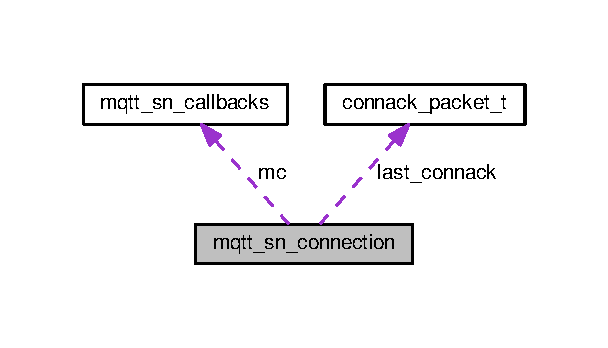
\includegraphics[width=292pt]{structmqtt__sn__connection__coll__graph}
\end{center}
\end{figure}
\subsection*{Membros públicos}
\begin{DoxyCompactItemize}
\item 
\hypertarget{structmqtt__sn__connection_ae825853452efa9c82bcaf89a50fef185}{{\bfseries L\+I\+S\+T\+\_\+\+S\+T\+R\+U\+C\+T} (requests)}\label{structmqtt__sn__connection_ae825853452efa9c82bcaf89a50fef185}

\end{DoxyCompactItemize}
\subsection*{Campos de Dados}
\begin{DoxyCompactItemize}
\item 
\hypertarget{structmqtt__sn__connection_ad171b51232de8bcdefba9d69f78b1f2b}{struct simple\+\_\+udp\+\_\+connection {\bfseries sock}}\label{structmqtt__sn__connection_ad171b51232de8bcdefba9d69f78b1f2b}

\item 
\hypertarget{structmqtt__sn__connection_ad5f06fa20c24cfc66b191395b1ef2b56}{uint16\+\_\+t {\bfseries next\+\_\+message\+\_\+id}}\label{structmqtt__sn__connection_ad5f06fa20c24cfc66b191395b1ef2b56}

\item 
\hypertarget{structmqtt__sn__connection_ae172b04589d6f7d3f097c263aa20def2}{struct ctimer {\bfseries receive\+\_\+timer}}\label{structmqtt__sn__connection_ae172b04589d6f7d3f097c263aa20def2}

\item 
\hypertarget{structmqtt__sn__connection_a39e71e16aa3e853f62aca3efc64f584c}{struct ctimer {\bfseries send\+\_\+timer}}\label{structmqtt__sn__connection_a39e71e16aa3e853f62aca3efc64f584c}

\item 
\hypertarget{structmqtt__sn__connection_afbbcf4a001540a2a6ec7f26aa6058661}{clock\+\_\+time\+\_\+t {\bfseries keep\+\_\+alive}}\label{structmqtt__sn__connection_afbbcf4a001540a2a6ec7f26aa6058661}

\item 
\hypertarget{structmqtt__sn__connection_aab30ea1c81fc48a2b08f5deaaafb2d4e}{\hyperlink{structconnack__packet__t}{connack\+\_\+packet\+\_\+t} {\bfseries last\+\_\+connack}}\label{structmqtt__sn__connection_aab30ea1c81fc48a2b08f5deaaafb2d4e}

\item 
\hypertarget{structmqtt__sn__connection_ab4524148feaa9d4fe5c15722114aedf5}{const char $\ast$ {\bfseries client\+\_\+id}}\label{structmqtt__sn__connection_ab4524148feaa9d4fe5c15722114aedf5}

\item 
\hypertarget{structmqtt__sn__connection_a47d5ca8da9b4b6faa46c933c51e64b53}{enum mqttsn\+\_\+connection\+\_\+status {\bfseries stat}}\label{structmqtt__sn__connection_a47d5ca8da9b4b6faa46c933c51e64b53}

\item 
\hypertarget{structmqtt__sn__connection_af32dc65bf9337fb62f3c5ee66c87222c}{uint8\+\_\+t {\bfseries connection\+\_\+retries}}\label{structmqtt__sn__connection_af32dc65bf9337fb62f3c5ee66c87222c}

\item 
\hypertarget{structmqtt__sn__connection_a9a77d0584b9412e8139bd1593e958bc6}{struct process $\ast$ {\bfseries client\+\_\+process}}\label{structmqtt__sn__connection_a9a77d0584b9412e8139bd1593e958bc6}

\item 
\hypertarget{structmqtt__sn__connection_a091e65235231be3ce1f4dbcfd746e727}{const struct \hyperlink{structmqtt__sn__callbacks}{mqtt\+\_\+sn\+\_\+callbacks} $\ast$ {\bfseries mc}}\label{structmqtt__sn__connection_a091e65235231be3ce1f4dbcfd746e727}

\end{DoxyCompactItemize}


A documentação para esta estrutura foi gerada a partir do seguinte ficheiro\+:\begin{DoxyCompactItemize}
\item 
mqtt-\/sn.\+h\end{DoxyCompactItemize}

\hypertarget{structmqtt__sn__request}{\section{Referência à estrutura mqtt\+\_\+sn\+\_\+request}
\label{structmqtt__sn__request}\index{mqtt\+\_\+sn\+\_\+request@{mqtt\+\_\+sn\+\_\+request}}
}


Diagrama de colaboração para mqtt\+\_\+sn\+\_\+request\+:
\subsection*{Atributos Públicos}
\begin{DoxyCompactItemize}
\item 
\hypertarget{structmqtt__sn__request_a195d599166341c09999ab1d2ecad64c1}{struct \hyperlink{structmqtt__sn__request}{mqtt\+\_\+sn\+\_\+request} $\ast$ {\bfseries next}}\label{structmqtt__sn__request_a195d599166341c09999ab1d2ecad64c1}

\item 
\hypertarget{structmqtt__sn__request_a3f7d86f3095ab0c85a2f72e117ad9e3d}{enum mqtt\+\_\+sn\+\_\+request\+\_\+state {\bfseries state}}\label{structmqtt__sn__request_a3f7d86f3095ab0c85a2f72e117ad9e3d}

\item 
\hypertarget{structmqtt__sn__request_afaf1a5289799f1ce19effa4201b2d266}{enum mqtt\+\_\+sn\+\_\+request\+\_\+type {\bfseries request\+\_\+type}}\label{structmqtt__sn__request_afaf1a5289799f1ce19effa4201b2d266}

\item 
\hypertarget{structmqtt__sn__request_a81cd1d5b87fc8c18593ae6c6593a8664}{uint16\+\_\+t {\bfseries msg\+\_\+id}}\label{structmqtt__sn__request_a81cd1d5b87fc8c18593ae6c6593a8664}

\item 
\hypertarget{structmqtt__sn__request_a49717cc0f847c6c4bb16b1b58322a0fe}{uint16\+\_\+t {\bfseries topic\+\_\+id}}\label{structmqtt__sn__request_a49717cc0f847c6c4bb16b1b58322a0fe}

\item 
\hypertarget{structmqtt__sn__request_af408a82a1506cbc1dbcc9a9b96799dc4}{uint8\+\_\+t {\bfseries return\+\_\+code}}\label{structmqtt__sn__request_af408a82a1506cbc1dbcc9a9b96799dc4}

\item 
\hypertarget{structmqtt__sn__request_a3bf0b52ec2d6ecdc167eb0e4cc15b62c}{struct pt {\bfseries pt}}\label{structmqtt__sn__request_a3bf0b52ec2d6ecdc167eb0e4cc15b62c}

\item 
\hypertarget{structmqtt__sn__request_af267ab5f24fe90e902976dd723775986}{struct ctimer {\bfseries t}}\label{structmqtt__sn__request_af267ab5f24fe90e902976dd723775986}

\end{DoxyCompactItemize}


A documentação para esta estrutura foi gerada a partir do seguinte ficheiro\+:\begin{DoxyCompactItemize}
\item 
mqtt-\/sn.\+h\end{DoxyCompactItemize}

\hypertarget{structmqttsn__topic}{\section{Referência à estrutura mqttsn\+\_\+topic}
\label{structmqttsn__topic}\index{mqttsn\+\_\+topic@{mqttsn\+\_\+topic}}
}
\subsection*{Campos de Dados}
\begin{DoxyCompactItemize}
\item 
\hypertarget{structmqttsn__topic_ad562f54acc5597130e0710c356963dff}{uint16\+\_\+t {\bfseries topic\+\_\+id}}\label{structmqttsn__topic_ad562f54acc5597130e0710c356963dff}

\item 
\hypertarget{structmqttsn__topic_a3682faf73e58b07c78516bab6be65755}{char {\bfseries topic\+\_\+name} \mbox{[}M\+Q\+T\+T\+\_\+\+S\+N\+\_\+\+M\+A\+X\+\_\+\+T\+O\+P\+I\+C\+\_\+\+L\+E\+N\+G\+T\+H\mbox{]}}\label{structmqttsn__topic_a3682faf73e58b07c78516bab6be65755}

\end{DoxyCompactItemize}


A documentação para esta estrutura foi gerada a partir do seguinte ficheiro\+:\begin{DoxyCompactItemize}
\item 
mqtt-\/sn.\+h\end{DoxyCompactItemize}

\hypertarget{structpuback__packet__t}{\section{Referência à estrutura puback\+\_\+packet\+\_\+t}
\label{structpuback__packet__t}\index{puback\+\_\+packet\+\_\+t@{puback\+\_\+packet\+\_\+t}}
}
\subsection*{Campos de Dados}
\begin{DoxyCompactItemize}
\item 
\hypertarget{structpuback__packet__t_ab2b3adeb2a67e656ff030b56727fd0ac}{uint8\+\_\+t {\bfseries length}}\label{structpuback__packet__t_ab2b3adeb2a67e656ff030b56727fd0ac}

\item 
\hypertarget{structpuback__packet__t_a1d127017fb298b889f4ba24752d08b8e}{uint8\+\_\+t {\bfseries type}}\label{structpuback__packet__t_a1d127017fb298b889f4ba24752d08b8e}

\item 
\hypertarget{structpuback__packet__t_ad562f54acc5597130e0710c356963dff}{uint16\+\_\+t {\bfseries topic\+\_\+id}}\label{structpuback__packet__t_ad562f54acc5597130e0710c356963dff}

\item 
\hypertarget{structpuback__packet__t_aa9c217c6e58cdb2408e2ffbe9425289d}{uint16\+\_\+t {\bfseries message\+\_\+id}}\label{structpuback__packet__t_aa9c217c6e58cdb2408e2ffbe9425289d}

\item 
\hypertarget{structpuback__packet__t_aa72e4a685c5a553897adf56e0e60a61e}{uint8\+\_\+t {\bfseries return\+\_\+code}}\label{structpuback__packet__t_aa72e4a685c5a553897adf56e0e60a61e}

\end{DoxyCompactItemize}


A documentação para esta estrutura foi gerada a partir do seguinte ficheiro\+:\begin{DoxyCompactItemize}
\item 
mqtt-\/sn.\+h\end{DoxyCompactItemize}

\hypertarget{structregack__packet__t}{\section{Referência à estrutura regack\+\_\+packet\+\_\+t}
\label{structregack__packet__t}\index{regack\+\_\+packet\+\_\+t@{regack\+\_\+packet\+\_\+t}}
}
\subsection*{Campos de Dados}
\begin{DoxyCompactItemize}
\item 
\hypertarget{structregack__packet__t_ab2b3adeb2a67e656ff030b56727fd0ac}{uint8\+\_\+t {\bfseries length}}\label{structregack__packet__t_ab2b3adeb2a67e656ff030b56727fd0ac}

\item 
\hypertarget{structregack__packet__t_a1d127017fb298b889f4ba24752d08b8e}{uint8\+\_\+t {\bfseries type}}\label{structregack__packet__t_a1d127017fb298b889f4ba24752d08b8e}

\item 
\hypertarget{structregack__packet__t_ad562f54acc5597130e0710c356963dff}{uint16\+\_\+t {\bfseries topic\+\_\+id}}\label{structregack__packet__t_ad562f54acc5597130e0710c356963dff}

\item 
\hypertarget{structregack__packet__t_aa9c217c6e58cdb2408e2ffbe9425289d}{uint16\+\_\+t {\bfseries message\+\_\+id}}\label{structregack__packet__t_aa9c217c6e58cdb2408e2ffbe9425289d}

\item 
\hypertarget{structregack__packet__t_aa72e4a685c5a553897adf56e0e60a61e}{uint8\+\_\+t {\bfseries return\+\_\+code}}\label{structregack__packet__t_aa72e4a685c5a553897adf56e0e60a61e}

\end{DoxyCompactItemize}


A documentação para esta estrutura foi gerada a partir do seguinte ficheiro\+:\begin{DoxyCompactItemize}
\item 
mqtt-\/sn.\+h\end{DoxyCompactItemize}

\hypertarget{structregister__packet__t}{\section{Referência à estrutura register\+\_\+packet\+\_\+t}
\label{structregister__packet__t}\index{register\+\_\+packet\+\_\+t@{register\+\_\+packet\+\_\+t}}
}
\subsection*{Atributos Públicos}
\begin{DoxyCompactItemize}
\item 
\hypertarget{structregister__packet__t_a24462876cab1ee115eab12d1f96f605f}{uint8\+\_\+t {\bfseries length}}\label{structregister__packet__t_a24462876cab1ee115eab12d1f96f605f}

\item 
\hypertarget{structregister__packet__t_a89183a1557a1c6422b0e6b9edf022941}{uint8\+\_\+t {\bfseries type}}\label{structregister__packet__t_a89183a1557a1c6422b0e6b9edf022941}

\item 
\hypertarget{structregister__packet__t_a2dd9b7da1b08d944eff685021eaefd26}{uint16\+\_\+t {\bfseries topic\+\_\+id}}\label{structregister__packet__t_a2dd9b7da1b08d944eff685021eaefd26}

\item 
\hypertarget{structregister__packet__t_af84a2324fa1e64ee1eafbd43e3580f4b}{uint16\+\_\+t {\bfseries message\+\_\+id}}\label{structregister__packet__t_af84a2324fa1e64ee1eafbd43e3580f4b}

\item 
\hypertarget{structregister__packet__t_a10223e5325f38eb2da99e06017220cb9}{char {\bfseries topic\+\_\+name} \mbox{[}M\+Q\+T\+T\+\_\+\+S\+N\+\_\+\+M\+A\+X\+\_\+\+T\+O\+P\+I\+C\+\_\+\+L\+E\+N\+G\+T\+H\mbox{]}}\label{structregister__packet__t_a10223e5325f38eb2da99e06017220cb9}

\end{DoxyCompactItemize}


A documentação para esta estrutura foi gerada a partir do seguinte ficheiro\+:\begin{DoxyCompactItemize}
\item 
mqtt-\/sn.\+h\end{DoxyCompactItemize}

\hypertarget{structtopic__map}{\section{Referência à estrutura topic\+\_\+map}
\label{structtopic__map}\index{topic\+\_\+map@{topic\+\_\+map}}
}


Diagrama de colaboração para topic\+\_\+map\+:
\subsection*{Atributos Públicos}
\begin{DoxyCompactItemize}
\item 
\hypertarget{structtopic__map_a4a4a7efc3ca6d975a7f51dccc600aaef}{uint16\+\_\+t {\bfseries topic\+\_\+id}}\label{structtopic__map_a4a4a7efc3ca6d975a7f51dccc600aaef}

\item 
\hypertarget{structtopic__map_ab8ec626e28a2e37244900cc9f2776b83}{char {\bfseries topic\+\_\+name} \mbox{[}M\+Q\+T\+T\+\_\+\+S\+N\+\_\+\+M\+A\+X\+\_\+\+T\+O\+P\+I\+C\+\_\+\+L\+E\+N\+G\+T\+H\mbox{]}}\label{structtopic__map_ab8ec626e28a2e37244900cc9f2776b83}

\item 
\hypertarget{structtopic__map_a4aa4dcf69f63404cf1f280fa21e197c0}{struct \hyperlink{structtopic__map}{topic\+\_\+map} $\ast$ {\bfseries next}}\label{structtopic__map_a4aa4dcf69f63404cf1f280fa21e197c0}

\end{DoxyCompactItemize}


A documentação para esta estrutura foi gerada a partir do seguinte ficheiro\+:\begin{DoxyCompactItemize}
\item 
mqtt-\/sn.\+h\end{DoxyCompactItemize}

\chapter{Documentação do ficheiro}
\hypertarget{main__core_8c}{\section{Referência ao ficheiro main\+\_\+core.\+c}
\label{main__core_8c}\index{main\+\_\+core.\+c@{main\+\_\+core.\+c}}
}


Arquivo principal do código fonte da rede mesh 6\+Lo\+W\+P\+A\+N ~\newline
 Para compilar este código, execute o makefile com o target desejado, por exemplo\+: ~\newline
 {\bfseries \char`\"{}make T\+A\+R\+G\+E\+T=srf06-\/cc26xx\char`\"{}} ~\newline
 Caso não reconheça qual o T\+A\+R\+G\+E\+T correto, utiliza o comando ~\newline
 {\bfseries \char`\"{}make targets\char`\"{}} ~\newline
 para listar os tags disponíveis.  


{\ttfamily \#include \char`\"{}contiki.\+h\char`\"{}}\\*
{\ttfamily \#include \char`\"{}lib/random.\+h\char`\"{}}\\*
{\ttfamily \#include \char`\"{}clock.\+h\char`\"{}}\\*
{\ttfamily \#include \char`\"{}sys/ctimer.\+h\char`\"{}}\\*
{\ttfamily \#include \char`\"{}net/ip/uip.\+h\char`\"{}}\\*
{\ttfamily \#include \char`\"{}net/ipv6/uip-\/ds6.\+h\char`\"{}}\\*
{\ttfamily \#include \char`\"{}mqtt\+\_\+sn.\+h\char`\"{}}\\*
{\ttfamily \#include \char`\"{}dev/leds.\+h\char`\"{}}\\*
{\ttfamily \#include \char`\"{}net/rime/rime.\+h\char`\"{}}\\*
{\ttfamily \#include \char`\"{}simple-\/udp.\+h\char`\"{}}\\*
{\ttfamily \#include $<$stdio.\+h$>$}\\*
{\ttfamily \#include $<$string.\+h$>$}\\*
{\ttfamily \#include $<$stdlib.\+h$>$}\\*
Diagrama de dependências de inclusão para main\+\_\+core.\+c\+:\nopagebreak
\begin{figure}[H]
\begin{center}
\leavevmode
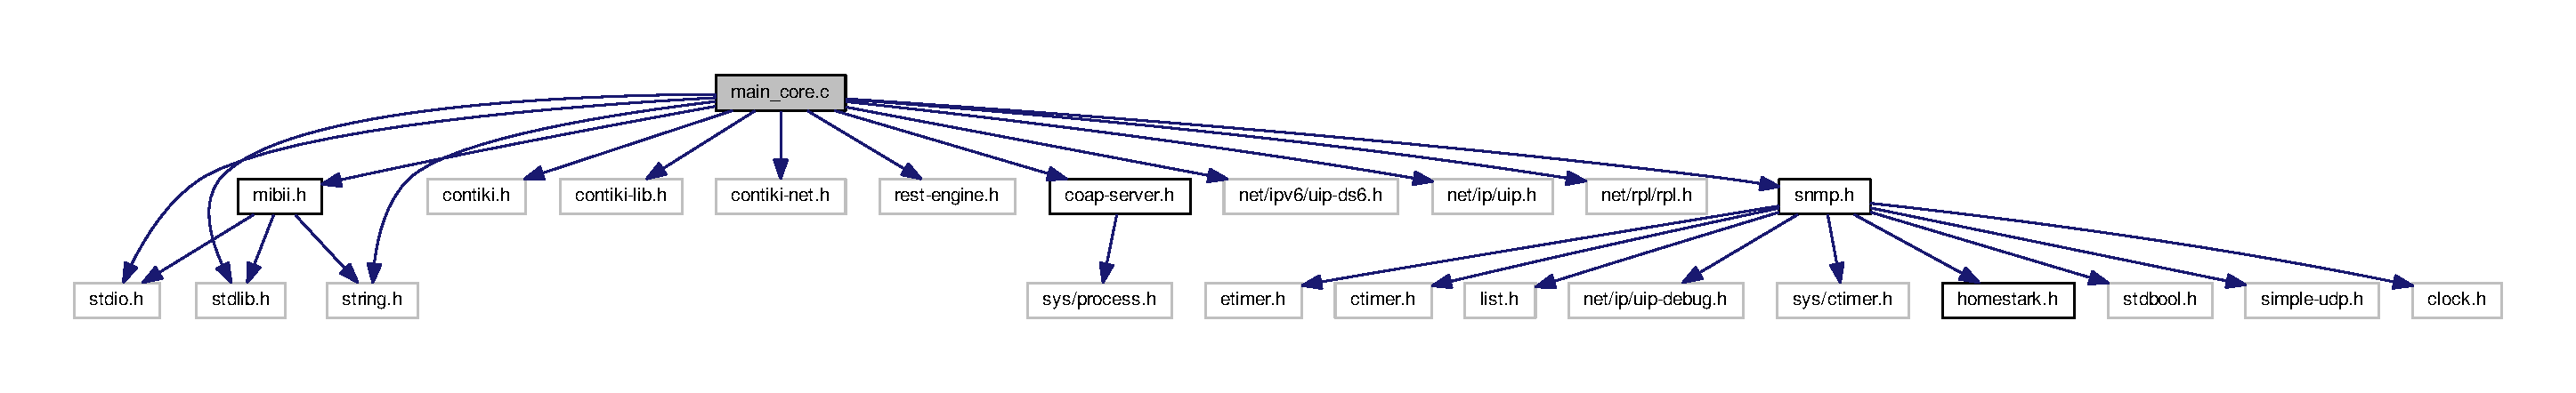
\includegraphics[width=350pt]{main__core_8c__incl}
\end{center}
\end{figure}
\subsection*{Funções}
\begin{DoxyCompactItemize}
\item 
\hypertarget{main__core_8c_a0a43995afea1479f111fbc2e35be0a7c}{void {\bfseries mqtt\+\_\+sn\+\_\+callback} (char $\ast$topic, char $\ast$message)}\label{main__core_8c_a0a43995afea1479f111fbc2e35be0a7c}

\item 
\hypertarget{main__core_8c_a271e0d9822452758a68f6e167c5209f8}{void {\bfseries init\+\_\+broker} (void)}\label{main__core_8c_a271e0d9822452758a68f6e167c5209f8}

\item 
\hypertarget{main__core_8c_a79354dfce54fd0bece29f8d443321b88}{{\bfseries P\+R\+O\+C\+E\+S\+S} (init\+\_\+system\+\_\+process,\char`\"{}\mbox{[}Contiki-\/O\+S\mbox{]} Iniciando sistema operacional\char`\"{})}\label{main__core_8c_a79354dfce54fd0bece29f8d443321b88}

\item 
\hypertarget{main__core_8c_a7683f5bdcb8cfbbb750ce92e76d1b7eb}{{\bfseries P\+R\+O\+C\+E\+S\+S\+\_\+\+T\+H\+R\+E\+A\+D} (init\+\_\+system\+\_\+process, ev, data)}\label{main__core_8c_a7683f5bdcb8cfbbb750ce92e76d1b7eb}

\end{DoxyCompactItemize}
\subsection*{Variáveis}
\begin{DoxyCompactItemize}
\item 
\hypertarget{main__core_8c_a5ca81254b9031056ba22742fb2252fd0}{\hyperlink{structmqtt__sn__con__t}{mqtt\+\_\+sn\+\_\+con\+\_\+t} {\bfseries mqtt\+\_\+sn\+\_\+connection}}\label{main__core_8c_a5ca81254b9031056ba22742fb2252fd0}

\item 
\hypertarget{main__core_8c_ac531a18312af7e29d65ccde0edd8b894}{A\+U\+T\+O\+S\+T\+A\+R\+T\+\_\+\+P\+R\+O\+C\+E\+S\+S\+E\+S \& {\bfseries init\+\_\+system\+\_\+process}}\label{main__core_8c_ac531a18312af7e29d65ccde0edd8b894}

\end{DoxyCompactItemize}


\subsection{Descrição detalhada}
Arquivo principal do código fonte da rede mesh 6\+Lo\+W\+P\+A\+N ~\newline
 Para compilar este código, execute o makefile com o target desejado, por exemplo\+: ~\newline
 {\bfseries \char`\"{}make T\+A\+R\+G\+E\+T=srf06-\/cc26xx\char`\"{}} ~\newline
 Caso não reconheça qual o T\+A\+R\+G\+E\+T correto, utiliza o comando ~\newline
 {\bfseries \char`\"{}make targets\char`\"{}} ~\newline
 para listar os tags disponíveis. 

\begin{DoxyAuthor}{Autor}
Ânderson Ignácio da Silva 
\end{DoxyAuthor}
\begin{DoxyDate}{Data}
19 Ago 2016 
\end{DoxyDate}
\begin{DoxySeeAlso}{Veja também}
\href{http://www.aignacio.com}{\tt http\+://www.\+aignacio.\+com} 
\end{DoxySeeAlso}

%--- End generated contents ---

% Index
\newpage
\phantomsection
\addcontentsline{toc}{chapter}{Índice}
\printindex

\end{document}
